\section{Decentralized Structured Architectures}
\label{section:structured}

This section focuses on the structured P2P architectures. The following
paragraphs contain a thorough discussion and analysis of the algorithms proposed
in the literature for dealing with the topology mismatch problem in such
architectures. In structured P2P systems, the construction of the routing tables
in every participating node determines the efficiency of message forwarding.
Therefore, routing tables that represent the underlying physical structure well
can achieve increased performance. For this reason, the proposed methods for
topology mismatch problem basically use different levels of proximity
information to optimize them towards this direction. The algorithms are here
categorised based the previous work done by
\cite{castro_proximitydht_2002,castro_topawareroute_2002,ratnasamy_openq_2002}.

\subsection{Algorithms for Structured Architectures}

%###############################################################################
%###############################################################################
%###############################################################################
%       GEGRAPHIC LAYOUT
%###############################################################################
%###############################################################################
%###############################################################################

%%%%%%%%%%%%%%%%%%%%%%%%%%%%%%%%%%%%%%%%%%%%%%%%%%%%%%%%%%%%%%%%%%%%%%%%%%%%%%%%
\subsubsection{Global Soft-State}

\begin{figure*}
\centering
  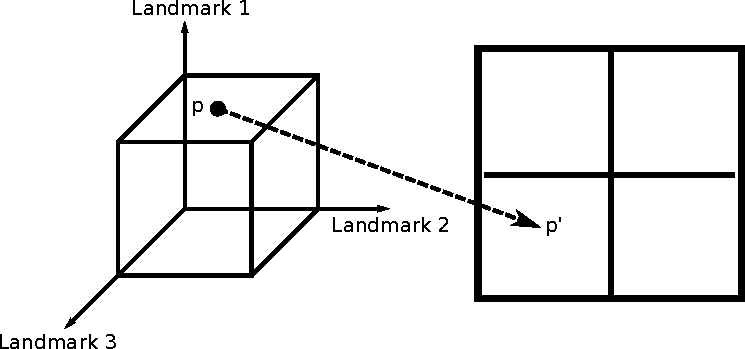
\includegraphics[scale=0.8]{img/algorithms/global_softstate}
\caption{(left) Position of $p$ in the space of $3$ landmarks. (right) Position
of $p$ on the map.}
\label{fig:global_softstate}
\end{figure*}

\textit{Global Soft-State} \cite{xu_globstate_2003} builds a global map to help
choose shorter routing paths, combining the landmark binning method and small
scale distance probes to reveal the proximity properties of the underlying
network to the overlay. Figure \ref{fig:global_softstate} presents the landmark
space and the mapping of the position of the nodes. This global view of the
state is made available to all nodes in order to help them find the best way to
route their messages. \textit{Global Soft-State} operates in two main stages,
generation and use of the proximity information. For generating the proximity
information a hybrid approach is proposed, which uses landmark clustering as a
preprocessing step in order to select a number of potential nearest neighbour
candidates and then refine the selection by incorporating a
round-trip-time-based scheme to ultimately choose the closest node. For using
the proximity information, the algorithm chooses a different path from the
classic gossiping approaches for constructing and maintaining the overlay. It is
based on landmark clustering for strategic placement of proximity information on
the overlay enabling any node to access such information using a landmark number
that reflects its physical position in the network. For various logical
regions\footnote{This might be a high-order zone in the eCAN\cite{xu_ecan_2002}
context or a set of nodes sharing a particular prefix in overlays such as
Pastry.} maps of physical information are built and published where each node
may appear in a maximum of $log\left( N \right)$ such maps. To dynamically adapt
to changing network conditions, a node subscribes to relevant \emph{soft states}
that utilize a notification system in order to initialize any necessary
neighbour re-selection.

Maintaining several host states at different layers, makes any content migration
costly. Additionally, the method does not make any continuing effort to remap
the overlay structure after a node successfully joins, in order to adapt its
  state to any condition change. Although this approach greatly reduces the
  routing latency to far nodes, it is unable to dynamically identify nodes that
  are close to routers and gateways in order to construct the secondary overlay.
Nevertheless, static recognition of such nodes is currently done based on BGP
reports and pre-chosen landmarks, sacrificing the self-organising attribute of
traditional DHTs.

%
% TODO: SOME DISCUSSION
%
% Xu \textit{et al.} \cite{xu_globstate_2003} state that there are three ways
% generating proximity information
%\begin{itemize}
% \item Expanding Ring Search\\
%Expanding ring search can be of two forms. First it can utilize the multicast
%infrastructure in the underlying network in order to emit its messages.
%Unfortunately such infrastructures are not widely deployed thus the
%implementations of this way of generating proximity information is limited to
%blindly flooding the neighbourhood to obtain reasonable results.
%
% \item Heuristics\\
%Heuristics are used in order to reduce the blindness of the expanding ring
%search and make realizations more efficient and effective. Unfortunately a
%common problem of all heuristic approaches is the local minimum pitfall in
%which
%the search might be caught into.
%
% \item Landmark Binning\\
%Landmark clustering is based on the view that nodes with similar distances to a
%set of predefined well-known landmark nodes are pretty likely of being close to
%each other. But this approach has its weaknesses as well, such as the fact that
%is a rather coarse grained approximation, therefore not particularly well
%suited
%for differentiating nodes within close distance to each other.
%
%\end{itemize}
%
%

%
% TODO: IN PAPER INTRODUCTION A DISCUSSION ABOUT
%TOPOLOGY-AWARE CAN
%
%Techniques to exploit topology information in overlay
%routing include geographic layout, proximity routing and
%proximity neighbor selection [3]. With geographic layout
%such as topology-aware CAN [12], the overlay structure is
%constrained by underlying network topology. This tech-
%nique, unfortunately, can create uneven distribution of
%nodes in the overlay, increasing the chances of overloading
%nodes and rendering the maintenance cost formidable. Our
%study shows that, for a typical 10,000-node topology-aware
%CAN, 5% nodes occupy 85-98% of the entire Cartesian
%space, and some nodes have to maintain 450-1500 neigh-
%bors. In Proximity routing, physical topology is not consid-
%ered when constructing the overlay.
%

\begin{center}
\begin{tabular}{ccc}
\emph{Efficiency} & \emph{Overhead} & \emph{Scalability} \\
\hline
% Unable to identify nodes that are close to routers but it can reduce routing
% latency to far away node by approximatelly 50-75%.
medium &
% maintenance of node states, subscriptions and notifications need global
% overview of the overlay resulting in high control overhead
high &
% Statically implemented sucrificing the the decentralised nature of DHTs and
% thus poorly scalling.
low
\end{tabular}
\end{center}

%%%%%%%%%%%%%%%%%%%%%%%%%%%%%%%%%%%%%%%%%%%%%%%%%%%%%%%%%%%%%%%%%%%%%%%%%%%%%%%%
\subsubsection{Mithos}
\emph{Mithos} \cite{waldvogel_mythos_2003} is a P2P protocol which incorporates
directed incremental probing to find near optimal node placement, and is
classified by its authors as an integration of geographic layout and proximity
routing overlay optimization methods.

The bootstrap phase of Mithos starts with a subset of existing members as the
first set of candidates, and while the iteratively closest nodes are detected by
probing the neighborhood, the candidate neighbor list is updated. In order to
avoid a local minima, Mithos probes all the neighbours within a two-hop distance
from the current minimum before concluding the process.

After finding its first neighbour, the newcomming peer is assigned an ID using
information gathered during the iterative neighbour selection phase. Virtual
coordinates are assigned to the newcomming peer by using the distances of two
closest nodes and their neighbours, so that Euclidean distances between the node
and all known hosts predict the network latency between them
\cite{cox_vivaldi_2004}. The benefit of these synthetic coordinates are that
they are explicitly used as the node's ID, and distance computations among nodes
can be done in ID space without requiring physical measurements.

The last step of the algorithm is the interconnection among neighbours. Mithos
uses a \emph{quadrant-based} mechanism according to which each node establishes
a link to the closest neighbour in each quadrant. During forwarding, the next
hop is performed towards a neighbour in the same quadrant as the final
destination. The newcoming node may not know of other neighbours in all
quadrants, therefore, the node first identifies neighbours in all quadrants
using a mechanism based on ideas similar to a perimeter walk\footnote{Used in
Greedy Perimeter Stateless Routing (GPSR) protocol.} and then improves the
results using parallel path processing by taking into account further geometric
properties of node relationships.

One major limitation of \textit{Mithos} is that the protocol cannot handle
dynamic arrivals and departures from the network, as is happens in mobile
networks.

%
% TODO: review this part
%
%In order to avoid local minima during neighbour detection, extensive probing
%  must be undertaken. In simulation, unfortunately, only very small-sized
% overlay topologies (of 200 to 1000 nodes) have been used and thus no safe
% conclusions can be made as for the behaviour of an extensively large,
% real-world p2p deployment of the scheme.

\begin{center}
\begin{tabular}{ccc}
\emph{Efficiency} & \emph{Overhead} & \emph{Scalability} \\
\hline
% It has very good results in reducing comunication latency among peers but its
% efficience is being constrained by the fact that the proximity is calculated
% at bootstrap, assigning virtual coordinates that are used througout of a
% nodes life cycle and thus the overlay is not adapting to a high-churn
% environment.
medium &
% Incrimental probing is applied in quadradants and in two-hop distance at each
% step that does not generate a lot o control overhead.
medium &
% It is constrained by the fact that the protocol does not respond to dynamic
% peer arrivals and departures
low
\end{tabular}
\end{center}

%%%%%%%%%%%%%%%%%%%%%%%%%%%%%%%%%%%%%%%%%%%%%%%%%%%%%%%%%%%%%%%%%%%%%%%%%%%%%%%%
\subsubsection{LAPTOP}
\emph{LAPTOP} \cite{wu_laptop_2007}, organises the overlay into a tree-based
hierarchy with main focus on reducing hops during message routing as well as
minimizing maintenance overhead. Additionally, a caching scheme is also
incorporated so as to further reduce routing table update costs. The authors
theoretically show that in LAPTOP routing path length is bounded by $O(log_d N)$
and node joining and leaving in the overlay network is bounded by
$O\left( d log_d N \right)$ hops in a balanced overlay tree, where $N$ is the
number of nodes, and $d$ is the maximum degree of each node. LAPTOP implements
the geographical layout approach  and constructs its layout in a self-organizing
and efficient fashion, by estimating the round-trip times to a small number of
nodes in the overlay network in order to make them roughly aware of their
physical distances among them.

Each node is assigned a dot-formated address (e.g 1.3.4). Each octet ranges from
$1$ to $d$, where $d$ is the maximum degree of the nodes. The assignment process
is done by appending a unique octet to the address of each nodes parent, while
root node is assigned address $1$.

%The protocol is based on four definitions.
%\begin{enumerate}
% \item The amplitude of all possible measured RTTs is devided into intervals.
%  Each node measures its distance to its parent and is assigned a label $L_i$
% where $i$ denotes the configurable RTT interval in which the measured distance
% falls into. A special kind of node, the root, is initially assigned the $L_1$
% label and maintains (as all $L_1$ nodes do) a list of other $L_1$ nodes in the
% overlay.
% \item Any node can have children with level lower than theirs, except an
%  $L_{max}$ node which can only have $L_{max}$ level children and only in the
% case when its parent has reached its maximum degree.
% \item Each node is assigned a dot-formated address (e.g 1.3.4). Each octet
% ranges from
% $1$ to $d$, where $d$ is the maximum degree of the nodes. The assignment
% process
% is done by appending a unique octet to the address of each nodes parent, while
% root node is assigned address $1$.
% \item For any descendant node $Y$ of a node $X$, the measured distance among
%  each other, must always be less than the lower bound of the RTT interval
% denoted by $X$'s label.
%\end{enumerate}
%

The routing scheme is similar to the longest-prefix IP matching scheme. At each
forwarding hop, any message travels up the tree until the first common ancestor
of both source and destination nodes is reached and then starts descending to
arrive to its target. During tree traversals, special entries in the routing
tables, called \emph{routing cache}, are maintained in order to increase routing
efficiency and achieve finer load balance. Caching enables a node to forward a
message to a better longest-prefix match than that of its direct ancestor making
a larger, quicker and more cost effective step through the overlay and toward
the destination. To improve scalability, the number of children nodes and the
size of the routing cache are limited. In terms of overlay maintenance, LAPTOP
incorporates a simple \emph{heartbeat}-based technique where each parent node is
responsible for monitoring its children.

%
%The newcommer $N$ locates the root node and the later responds with a list of
%  $L_1$ nodes. $N$ then probes each of the $L_1$ nodes in search for the
% closest one. If the measured RTT to the closest $L_1$ falls into the first
% interval then the newcommer becomes a $L_1$ node as well. Otherwise node $N$
% sets the closest $L_1$ node as its potential parent node. This potential
% parent becomes the actual parent if it does not have any other children. If it
% has, $N$ gets a list of these $L_i$ nodes and by measuring the RTT to each of
% them tries to spot a new potential parent in order to repeat the above
% process.
%

% At join process the newcomming node is assigned its level label as well as its
% address by its parent node. Additionally, it initializes its routing table
%(with normal and caching entries) as it traverses the overlay in search for
%its parent node.  During a graceful departure, the referred node checks for
%children in the overlay. If it does not have any, it simply notifies its
%parent and leaves. If it has, it selects the child node with the lowest
%round-trip time to it in order to take its place so that the locality
%property is preserved. On the other hand, in the case of an arbitrary
%failure, after the children of the failed node detect their parent's absence
%(throught the aformentioned heartbeat mechanism), they start emmiting special
%messages to their grandparent node (the address of which is stored during
%join process}. In case of no response from the grandparent node, the children
%invoke the joining process to detect their new parent node.The parent of the
%failed node, aggregates the notifications from the above children nodes for a
%period of time, and then chooses the one with the lowest level label as the
%takeover node. Potential ties are broken by favouring the lower RTT. The
%parent of the failed node, finally informs accordingly all the children about
%the change in the hierarchy.

%%%%%%%%%%%%%%%%%%%%%%%%%%%%%%%%%%%%%%%%%%%%%%%%%%%%%%%%%%%%%%%%%%%%%%%%%%%%%%%%
%
% TODO: HERE STRUCTURED LANDMARK BINING APPROCH LIES
%
%Assuming a structured approach based on CAN\cite{ratnasamy_can_2001} and $m$
% landmark nodes. The coordinate space is then partitioned into $m!$ equally
%sized portions, each corresonding to a single ordering of the landmarks. To do
%this, the first dimension is divided into $m$ areas each of which is furtherly
%divided (second dimension) into $m - 1$ sections and so on. Having set this $m$
%dimensional space, at joining time, a node measures the delay to the set of
%landmarks in order to determine its associated bin and thus position itself in
%that portion of the coordinate space associated with its landmark ordering.
%Even though this scheme can
%


\begin{center}
\begin{tabular}{ccc}
\emph{Efficiency} & \emph{Overhead} & \emph{Scalability} \\
\hline
% It minimises routing length, but may suffer load imbalance since nodes higher
% in the tree hierarchy are more likely to route most of the messages in the
% overlay.
medium &
% Heartbeat approach incurs extra control overhead to the network. Fortunatelly
% involves only the parent and the children of the departing/failing node.
% nodes.
low &
% Seems to scale nicely from 10K- to 1M-node testbeds.
high
\end{tabular}
\end{center}



%###############################################################################
%###############################################################################
%###############################################################################
%       PROXIMITY ROUTING
%###############################################################################
%###############################################################################
%###############################################################################


%%%%%%%%%%%%%%%%%%%%%%%%%%%%%%%%%%%%%%%%%%%%%%%%%%%%%%%%%%%%%%%%%%%%%%%%%%%%%%%%
\subsubsection{Proximity in Kademlia}
% Before discussing {\em Proximity in Kademlia}, it would be helpful to briefly
% summarize the highlights about the {\em Kademlia} protocol. {\em Kademlia}
% \cite{maymounkov_kademlia_2002} is a distributed hash table (DHT) based
% protocol for P2P networks, which uses an iteration based lookup algorithm. The
% protocol uses the standard $160$ bit ID system for nodes and locates the nodes
% in a prefix binary tree, where IDs are used as prefixes. The iterative lookup
% operations are done over this prefix binary tree, which converges to
%logarithmic
% lookup times. The ID's are assigned randomly, therefore in Kademlia, there is
%no
% proximity control, which results in inefficient use of the underlying network
% during lookup and retrieve operations.

\emph{Proximity in Kademlia} \cite{kaune_pkad_2008} introduces proximity
controls over the vanilla Kademlia protocol's random ID assignment, in order to
optimize the underlying network usage of the protocol. The work in this paper
can also be considered, as a more generic study over building proximity in the
context of iterative lookup algorithms. Focus is given on both the overlay and
the underlaying tiers in the sense that in the first improves the routing
performance according to a cost metric that is provided by the later and
quantifies the suitability of establishing a communication link between peers as
a cost function, based on the used proximity criteria (RTT, ISP locality, etc.).
%An underlay metric provides information about the underlay network. The paper
%  distingushes between three kinds of possibilities to quantify it:
%\begin{itemize}
% \item Using measurements gained by previous lookups
% \item Using measurements acquired by other peers or jointly calculated with
%  others
% \item Using a local database to look up information
%\end{itemize}
The paper proposes two approaches for overlay optimisation. One falling into
{\em proximity routing} and the other on {\em proximity neighbour selection}
approaches overlay optimization techiques for exploiting proximity. For the
first, the goal is in choosing the best next hop during routing a message. Due
to the fact that the routing in Kademlia is iterative, it is the initiator of
the lookup that chooses each next hop from a set of candidate nodes. Standard
Kedemlia always chooses the closest node with respect to the XOR metric but with
proximity routing selection, Kademlia chooses the one with the smallest underlay
metric cost. Thus, as in all such approaches, there is a trade-off between the
overlay and underlay distances.

Toward the enhancement of traffic locality, the authors also use information
from the MaxMind GeoIP database\footnote{MaxMind Geolocation Technology.
http://www.maxmind.com} to retrieve proximity information of a given peer based
on its region, country, or ISP location, and use this information to form
clusters of nearby peers. An alternative method could also be the use of Vivaldi
coordinates \cite{cox_vivaldi_2004}. However, authors report that clustering
approach performs better than Vivaldi protocol based on their experiments.
Authors also report that {\em Proximity routing} protocol successfully worked
with the Kademlia protocol and improved the locality of the connections over
peers.

As already mentioned the paper proposes \emph{proximity neighbour selection}
method, as well, for overlay optimisation. The goal, according to this, is to
keep peers with the least contact cost in the routing table. As Kademlia
constantly learns new peers (incoming requests, through iterative lookup) no
special algorithm for searching more cost effective peers is necessary and
simply choose the best peers seen so far.

\begin{center}
\begin{tabular}{ccc}
\emph{Efficiency} & \emph{Overhead} & \emph{Scalability} \\
\hline
% Uses static information to cluster nodes which is not the most efficient
% approach in dynamic systems
medium &
% 
medium &
%
medium
\end{tabular}
\end{center}

%%%%%%%%%%%%%%%%%%%%%%%%%%%%%%%%%%%%%%%%%%%%%%%%%%%%%%%%%%%%%%%%%%%%%%%%%%%%%%%%
\subsubsection{CHOord considering Proximity on IPv6 (CHOP6)}
\emph{CHOP6} \cite{morimoto_chop6_2007} roughly estimates the proximity among
nodes by exploiting the IPv6 address format and RTT information if available.
The proximity estimation is achieved by introducing a 64-bit ID scheme in which
the least significant bit part is the IPv6 global routing prefix and thus
enabling a longest prefix match scheme. The protocol is designed based on the
observation that it is possible to estimate a node's geographical location by
simply examining the upper 32-bits of its IPv6 address. Moreover, similar to
Chord, CHOP6 uses a finger table, whose entries hold more than
one candidate node.

%
%\paragraph{}
% There are three cases in which a node chooses the next hop according to
% information it posseses.
%\begin{itemize}
% \item When no information about RTT is available candidate next hops, the
%  sender just selects a node in the finger table entry which shares the longest
% prefix with the destination.
% \item There is another possibility that after some communication with other
%  nodes, the source node should know of the RTTs to some of the nodes in finger
% table entry. In this case, the source node chooses the one with the smallest
% RTT with propability $p$. If there is a node with no measured RTT then the
% sender can select such a node with probability $1 - p$
% \item In this last case the source node has already communicated with all
%  candidate node in the finger table entry. Thus, the node selects the node
% whose RTT is the smallest with probability $p$, the one with the second
% smallest with probability $q$ and so on, where $0 \leq \ldots < r < q < p < 1$
% and $p+q+r+\ldots \leq 1$
%\end{itemize}
%

\begin{center}
\begin{tabular}{ccc}
\emph{Efficiency} & \emph{Overhead} & \emph{Scalability} \\
\hline
% Simple approach that exploits proximity but it is coarse grained and thus not
% efficient.
low &
%
low &
%
medium
\end{tabular}
\end{center}

%%%%%%%%%%%%%%%%%%%%%%%%%%%%%%%%%%%%%%%%%%%%%%%%%%%%%%%%%%%%%%%%%%%%%%%%%%%%%%%%
\subsubsection{T2MC}
T2MC \cite{shi_t2mc_2008} uses traceroute logs to detect different autonomous
systems and cluster close by peers, thus reducing redundant traffic that crosses
autonomous system boundaries. T2MC uses a customized k-mean classification
algorithm with $k=2$ to perform the classification, and exploits the stable
structure of the Internet routers to guide clustering. The peer chooses the
minimum and maximum Latency results from the traceroute to initialize the
centroinds of two sets. Then the peer calculates, for all hops allong its
tracerouted path, the absolute distance to these centroids of both sets and
assigns the routers to that centroid with which it has the smaller absolute
distance. After that, the mean and variance values are calculated and if the
variance is larger than a predefined threshold then the algorithm sets the two
latency mean values as new centroids for the two sets and loops again.
Ultimately peer will end up with two sets having the minimum intra-set variance.
The peer, then, chooses the router from the second set with the minimum hops
attribute and sets it as a threshold. The selected router and all others whose
hops attribute is larger than the threshold are classified as \emph{remote}
router cluster. The remaining are classified as \emph{near}. From the near
class, the peer chooses the one with maximum hops attribute as its edge router,
and registers it along with the all the near cluster into the DHT of the P2P
overlay. As new peers join the network, those that share the same edge router
or any of the members of the near router clustersm there would gather to form a
close peer cluster. As Edge routers can provide more valuable information than
other members of the near set, T2MC was designed to prioritize interaction of
peers and edge gateways.

%
% TODO: SOME DISCUSSION
%
%The use of Traceroute as a tool for implementing the distance measuring
%infrastructure raise concearns about its efficiency and scalability. Being,
%primarilly, a network diagnostic utility,
% Even though traceroute provides detailed information about the network
% structure, its excessive use creates additional overhead that stresses further
% the overall network infrastructure. This forces network administrators to
% disable its support from the routers they manage, thus jeopardizing the
% effectiveness of the T2MC algorithm.
%


\begin{center}
\begin{tabular}{ccc}
\emph{Efficiency} & \emph{Overhead} & \emph{Scalability} \\
\hline
% The efficiency of choosing close by peers is very good and reported almost
% 65\% better than that of GNP (and thus generally of static landmarking as a
% whole)
high &
% traceroute is a very heavy tool and thus incurs excessive burden to the
% network resourses.
high &
% Traceroute is categorised as too heavy-weighted and intrucive for use in a
% larger scale system \cite{ratnasamy_binning_2002}. Additionally, disabling
% ICMP is a common administrative policy for edge sites to enforce security,
% while dumping BGP routing tables\cite{krishnamurthy_bgpclust_2000} is not
% directly available to the application layer.
low
\end{tabular}
\end{center}

%%%%%%%%%%%%%%%%%%%%%%%%%%%%%%%%%%%%%%%%%%%%%%%%%%%%%%%%%%%%%%%%%%%%%%%%%%%%%%%%
\subsubsection{PChord}
\emph{PChord}\cite{hong_pchord_2005} is a based on the Chord DHT which adds
proximity routing into its routing mechanism. The main modification over the
vanilla Chord is the inclusion of a \emph{proximity list} into its routing table
so that the next hop is decided based not only by considering best progress
towards the key, but on the physical proximity of the candidate nodes as well.
The list is, at join time, empty but as the PChord node starts to interact with
other nodes it applies a heuristic mechanism to fill up the list. Entries are
dynamicaly added or removed as the network state changes. The overlay
maintenance cost can be considered similar to Chord's since besides node
join/leave and cost of finger table entries heartbeat, PChord adds heartbeat of
nodes inside the proximity list but since this list always contains nodes with
the lowest RTT the added cost is kept to a minimal.

Due to the fact that, with each step, there is always progress towards the
target node in the ID space, PChord will result in a reduced hop number than
Chord, since each hop in PChord is larger or at least equal in the key space.
Passing through proximity links in the underlaying network means reduced routing
cost. Additionally, if the number of entries in the proximity list is the same
as the number of network partitions, PChord prevents hops from jumping in and
out the network partition the current node belongs to.

% TODO: SOME DISCUSSION
% TODO: NEEDS REWORDING
% PChord’s main routing optimizations are of less overlay hops, passing
% proximity links of the underly network and passing the same network partition
% only once in the routing path, which directly results in the lower RDP of
% routing efficiency. Meanwhile, PChord keeps light-weightmaintenance cost as
% Chord does.


\begin{center}
\begin{tabular}{ccc}
\emph{Efficiency} & \emph{Overhead} & \emph{Scalability} \\
\hline
% Small decrease in needed overlay hops per object publishing
medium &
% The are heartbeat mechanism for both finger table and proximity list adds a
% burden to the network by default. But the overall overhead is decreased as
% the proximity list becomes longer.
medium &
% Improvement of routing is achieved with more object pointers helping to
% shorten the routing path of object querying. When the distance of query source
% to target is far away both Chord and PChord achieve the average hop number to
% not increase.
high
\end{tabular}
\end{center}

%%%%%%%%%%%%%%%%%%%%%%%%%%%%%%%%%%%%%%%%%%%%%%%%%%%%%%%%%%%%%%%%%%%%%%%%%%%%%%%%
\subsubsection{AChord}
\emph{AChord} \cite{dao_achord_2006} uses IPv6's anycast mechanism in order to
releave the protocol from complex joining procedures, and achieve high accuracy
of network proximity giving high routing efficiency, Anycast delivers a message
comming from the outside of an anycast group to the physicaly closest node in
that group. AChord organizes all nodes participating in the overlay network into
an anycast group. Any joining node comes outside of that group and, thus, is
automaticaly forwarded to the physicaly nearest node in order to bootstrap,
avoiding the need to, explicitly, maintain such nodes, and the effort of finding
a way of locating the physically nearest among them. The ID of the new comming
node is computed based on the ID of the bootstrap node and the bootstrap's
predecessor in a way that the constructed ID will be positioned between the
aformentioned two. After joining, the finger table is build the same way as in
the Chord protocol. Moreover, additional nodes are maintained in a structure
called \emph{neighbourship table} which stores information about the closest
known node. The routing decision is made by using both the neighbourship and
the finger table. The authors claim this to be a lightweight approach that
requires few changes to Chord in order not to affecting its own advantageous
characteristics.

% TODO: MAYBE REVIEW THE EVALUATION
\begin{center}
\begin{tabular}{ccc}
\emph{Efficiency} & \emph{Overhead} & \emph{Scalability} \\
\hline
% good routing efficiency
medium &
% Releaves the system from joining overhead and topology aware ID construction
% but doubles the information needed to be stored and maintained by the
% introduction of neighbouring table
medium &
% assumes the operation of ideal underlying anycast mechanism (meaning that
% outside messages are always routed to the nearest node which in the current
% Internet, this is not always feasible. Moreover, is designed on the basis of
% IPv6 protocol which is not widely operational yet.
medium
\end{tabular}
\end{center}

%%%%%%%%%%%%%%%%%%%%%%%%%%%%%%%%%%%%%%%%%%%%%%%%%%%%%%%%%%%%%%%%%%%%%%%%%%%%%%%%
\subsubsection{Chord6}
\emph{Chord6} \cite{xiong_chord6_2005} is another Chord variant that tries to
exploit the hierarchical features of IPv6 in order to create a substrate that
reduces inter-domain traffic between service providers. The difference between
Chord6 and Chord the identifier definition. Therefore, the approach can be
easily portable to other DHTs such as CAN, Pastry and Tapestry. In Chord6 the
identifier contains two parts: the higher bits are obtained by hashing the
node's IPv6 address prefix of specific length, while the remaining lower bits
are the hash value of the rest of that IPv6 address. As a result of this
assignment, nodes in a domain will be mapped onto a continuous key space on the
overlay network, which avoids unnecessary message forwarding across different
service providers, thus minimising overall routing cost.

\begin{center}
\begin{tabular}{ccc}
\emph{Efficiency} & \emph{Overhead} & \emph{Scalability} \\
\hline
% Can reduce intra-domain average path length but even though nodes in the same
% domain would have close identifiers, nodes in two close domains may have very
% different ones reducing the overal efficience of the approach in general when
% considering inter-domain average path length.
low &
% The construction of the identifier space is done at node join and in an
% independent fashion involving the application of two hash functions meaning
% resulting in low overhead stress to the network and its nodes.
low &
% Is designed on the basis of IPv6 protocol which is not widely operational yet.
medium
\end{tabular}
\end{center}

%###############################################################################
%###############################################################################
%###############################################################################
%       PROXIMITY NEIGHBOUR SELECTION
%###############################################################################
%###############################################################################
%###############################################################################

%%%%%%%%%%%%%%%%%%%%%%%%%%%%%%%%%%%%%%%%%%%%%%%%%%%%%%%%%%%%%%%%%%%%%%%%%%%%%%%%
\subsubsection{DHT-PNS}
The work in \cite{hancong_pnsbased_2006} propose a proximity neighbour selection
scheme on top of the Chord DHT. The main goal is to use proximity information
to group physically close by nodes as neighbours in the DHT table. In order to
detect proximity, virtual network coordinates of peers are used, by using the
Vivaldi protocol \cite{cox_vivaldi_2004}. The virtual coordinates are then used
by the nodes to map to identifier space in the DHT. The space is partitioned
using a \emph{concentric circle clustering scheme} where successive cycles of
radiuses $\rho$, $2\rho$, $3\rho$ and so on, are constructed. Then the formed
annuluses are divided into $2\chi-1$ \emph{sectors}, where $\chi$ denotes the
sequence number of the annulus starting from $\chi = 1$ for the centre cycle. It
is proved in the paper, that this way each sector occupies the same area as does
the center cycle. Assuming uniform node distribution, this characteristic,
favours a more load balanced clustering operation. Every sector in this $2d$
coordinate space is mapped to a unique \emph{region} in the DHT space forming a
multi-layer node identifier space.  Thus, any nodes that belong to the same
sector, are mapped to the same region as well, preserving their proximity
relationship unveiled by the use of the Vivaldi protocol. The individual pieces
are mapped to the identifier space uniquely, allowing logarithmic lookup
operations with high probability on Chord. The system described in the previous
section allows any node to obtain its DHT key and its region key, in a fully
distributed manner, just by applying a consistent hash function. Using an RPC
call in Chord, the node can obtain the region's master node, called
\emph{Cluster Node (CN)} which is responsible for clustering the nodes belonging
in the same sector or region with that of the node at hand. An additional RPC
call, registers it to its corresponding region and publishes its information,
through the special peer CN. The node can, additionaly, ask CN for other
nodes that have previously joined the region in order to add them into its
neighbour set for future routing table optimization. Even in the case when no
neighbour is detected in the current region, the search is expanded to adjasent
regions and towards an upper layer identifier space until one is found or the
first layer reached.

% TODO: MAYBE REVIEW THE EVALUATION
\begin{center}
\begin{tabular}{ccc}
\emph{Efficiency} & \emph{Overhead} & \emph{Scalability} \\
\hline
%
medium &
%
medium &
%
medium
\end{tabular}
\end{center}

%%%%%%%%%%%%%%%%%%%%%%%%%%%%%%%%%%%%%%%%%%%%%%%%%%%%%%%%%%%%%%%%%%%%%%%%%%%%%%%%
\subsubsection{Quasi-Chord}
The approach that is proposed by Sun and Zhang in \cite{sun_quasi_2008}, tries
to address the topology mismatch problem, at the construction phase of the
Chord identifier cycle, on the the basis of underlying topology information.
The proposed model constructs the \emph{Quasi-Chord} ovelay network in three
steps. First, each host acquires its coordinates in the geometric space
utilizing the \emph{global network position (GNP)} protocol \cite{ng_gnp_2001}.
Second, using the \emph{Cantor space filling curve}, the $2$-dimensional space
is converted to a $1$-dimensional one, used in the last, third, step to build
the Quasi-Chord circle according to the host's Cantor value. In Quasi-Chord
each node stores 2 finger tables; one clockwise and one counter-clockwise.

%In the following paragraphs, these steps are furtherly discussed.
%
%\paragraph{GNP coordinates}
%First of all the host must be positioned in the geometric space. The algoritm
%  models the P2P network with a well defined distance function in such a way,
% it can predict, with high accuracy, the distance between any two points in the
% space by just evaluating the output of the distance function on the
% coordinates of these points. This is accomplished with the \emph{global
% network position (GNP)} protocol which\begin{inparaenum}[\itshape i\upshape)]
%  \item creates a reference set of $N$ landmark nodes so as to minimize the
%  error of ICMP measured distances and coordinate computed ones between them,
% and then
%  \item each host is able to measure its round-trip times to the $N$ Landmarks
% in order to compute its own coordinates.
%\end{inparaenum}
%
%\paragraph{Cantor SPF}
%After the $2$-d coordinates are set, in the next stage of the algorithn, each
%  participating peer is assigned a Cantor value, according to the application
% of a \emph{space filling curve} on the coordinate space. (TODO: add figure).
% This results in the conversion of the $2$-dimensional space to a
% $1$-dimensional Cantor space that can more easily be more mapped to the Chord
% hierarchy.
%
%\paragraph{Quasi-Chord construction}
%As can intuitively be infered by observing the Cantor chart, close-by nodes in
%  the physical layer, are more likely to have similar Cantor values. This
% attribute is exploited in order to construct a topology-aware identifier space
% for the Chord DHT. The cycle is constructed by sorting nodes in ascending
% order. Each host maintains 2 finger tables, one for clockwise and one for
% counter-clockwise stepping. This helps with the connectivity of the network
% because its not allowed to connect the first node with the last one since this
% will incur heavy traffic to the later\footnote{After all their Cantor values
% denote that they are actually the furthest of each other.}.
%

%
% TODO: SOME DISCUSSION
%       NEEDS DOUBLECHECK
%
%The disadvantage of the algorithm is that the coordinate assignment in the
%  first stage is backed by a not fully distributed landmark-based algorithm.
% Moreover the Quasi-Chord model build-up is making an indirect assumption of a
% maximum number of allowable hosts since it is constructed. Last but not least
% the doubling of the required routing information which needs to be created and
% maintained is an additional negative point to the efficiency and the
% scallability of the algorithm.
%

\begin{center}
\begin{tabular}{ccc}
\emph{Efficiency} & \emph{Overhead} & \emph{Scalability} \\
\hline
% The algorithm shows to reduce end-to-end delay as well as not produce
% duplicates of messages.
medium &
% The overhead is more compared to vanilla chord since mapping of 2-dimensional
% space to 1-demensional with Cantor SPF adds some extra burden in time
% complexity. Also the addition of the couter-clockwise finger table doubles the
% data, per se, needed to be stored and maintained.
high &
% The GNP system is a static landmark approach making things not fully
% distributed and thus constrain the model's scalability.
medium
\end{tabular}
\end{center}

%%%%%%%%%%%%%%%%%%%%%%%%%%%%%%%%%%%%%%%%%%%%%%%%%%%%%%%%%%%%%%%%%%%%%%%%%%%%%%%%
\subsubsection{IP-based Clustering (IPBC)}
Proximity neighbour selection algorithms use probing and other techniques to
detect proximity. However, such methods are either not precise enough, or
overload the network. \emph{IP-based clustering} \cite{karwaczynski_ipbc_2007}
is a proximity neighbour selection based algorithm in which the authors propose
to use the IP address prefixes (16 bit for IPv4) in order to detect proximity.
\cite{freedman_iploc_2005} states that $97\%$ of prefixes larger than $24$ bits
belong to a single geographical location. However, using less number of bits
creates less precise results and more number of bits increase the burden on the
network and reduce the possible number of neighbours. Therefore, a careful
selection is required in terms of performance/accuracy tradeoff. IP-based
Clustering generates a key and its prefix and stores the later in the DHT
itself, so that any newly joining nodes with the same IP prefix can query it and
identify all the neighbours with the same one relatively easy. Nodes
periodically update their entries in the DHT by removing those who leave, or
those who has been timed out with no further activity detected from the node.

% Moreover, observing the
% \emph{IANA IPv4 Address Space Registry} we can infer that, since blocks of
% consecutive octet prefixes are assigned to the same Regional Internet
% Registries (RIRs), nodes inside will be physicaly close to each other.

%
% In order to be published in the overlay, each node is first assigned a
% unique identifier and subsequently generates a key by hashing a fixed-length
% prefix of its IP. Authors argue on the prefix length to be used, as there is a
% thin balance between reducing the propability of finding closer nodes by
% adopting a long prefix and overload nodes that are responsible for information
% published by many peers when chosing to hash a short one. Their verdict is for
% the use of a 16-bit wide prefix for real world systems deployed in an Internet
% scale. In either case, ID and IP is then stored in the DHT using this
% generated key. This way, any node, at any time (either at join time or during
% peer lifetime for topology adaptation) can acquire information about close-by
% nodes just by quering thde DHT for a specific key. Moreover, the algorithm
% takes care of the freshness of the proximity information in two ways. First,
% the advertising nodes themselves periodically update their advertisements or
% when they voluntarily leave the overlay, they explicitly remove their data. On
% the other hand, in case of a failure each publication is assigned an
% expiration time, and thus ultimately removed by the DHT maintenance
%mechanisms.
%

\begin{center}
\begin{tabular}{ccc}
\emph{Efficiency} & \emph{Overhead} & \emph{Scalability} \\
\hline
% The efficiency of proximity detection through the prefix matching technique
% is caught in a vicious cycle with the storage space needed for DHT object
% publishing (how many bits will be used for either)
low &
% The overhead for detecting proximity is only comparison of prefixes
low &
%
medium
\end{tabular}
\end{center}

%%%%%%%%%%%%%%%%%%%%%%%%%%%%%%%%%%%%%%%%%%%%%%%%%%%%%%%%%%%%%%%%%%%%%%%%%%%%%%%%
\subsubsection{Cone}
\emph{Cone} \cite{wang_cone_2007} extends Chord using proximity neighbour
selection topology optimization algorithm. The proximity information is
generated using landmarks and round-trip-time-based distances to landmarks.
Cone uses a two-layered identifier space. The first, named Chord-layer
identifier, denoted as $Id_{Chord}$, is the same as in Chord. The second is the
Cone-layer identifier, $Id_{Cone}$ which is constructed by two component
identifiers. The first, known as \emph{group identifier (gid)} denotes a
relevant group the node belongs to while the second, namely \emph{local
identifier (lid)} indicates the local identifier within the group. The group
concept, which is introduced here, is a way of dividing nodes according to a
common $Id_{Chord}$ prefix.  The structure of a Cone overlay, retains the
Chord's circular topology. The difference lies on the fact that, now, two rings
are created. A big ring, where nodes with the same \emph{gid} are arranged at
each position. Each of these positions are a smaller ring for the particular
group's \emph{lid}s. The routing is achieved in both clockwise and
counter-clockwise directions in the big-ring, for which two routing tables are
maintained, namely \emph{front} and \emph{back} finger tables. Entries in these
tables, display physical network proximity with the current node. Moreover, a
third table called \emph{group} maintains information about other online peers
within the current node's group in a way that entries are now close in the ID
space.

%
%Routing in Cone, comprises of the inter-group algoritm and the intra-group
%  algorithm. First the group of nodes to which the desired key lies is
% detected, exploiting physical proximity information (front and back finger
% tables). Second during the next and last hop, the message is forwarded to the
% exact node that contains the desired key.
%

\begin{center}
\begin{tabular}{ccc}
\emph{Efficiency} & \emph{Overhead} & \emph{Scalability} \\
\hline
% The result of experiments show that the Cone, compared with Chord, has obvious
% improved on the delay of route and the hops of overlay networks…
medium &
% The approach incorporates a static landmark + RTT to these landmarks in order
% to exploit proximity information thus incurring low overall additional
% operational overhead but imposing extra stress to the landmarks themselves 
medium &
% landmark based approaches are not full distributed thus not smoothly scalable.
medium
\end{tabular}
\end{center}

%%%%%%%%%%%%%%%%%%%%%%%%%%%%%%%%%%%%%%%%%%%%%%%%%%%%%%%%%%%%%%%%%%%%%%%%%%%%%%%%
\subsubsection{DynaMo}
\emph{DynaMO} \cite{winter_dynamo_2004} tries to build an overlay that not only 
considers physical proximity among peers but their mobility attributes as well.
DynaMO is based on a Pastry overlay network and this was a preety concious
choice, by the authors, basically because of Pastry's built-in locality
heuristics which are thoroughly analysed in the in the literature
\cite{castro_proximityp2p_2002} providing good backround against which to test
and compare their results. In order to adapt to mobile, ad-hoc networks,
though, special care has been put to the maintenance of an even overlay ID
distribution so that hot-spots are avoided. DynaMO dictates a newcoming node to
gather information concerning its physical neighbourhood and uses it to assign
itself an appropriate overlay ID. DynaMO tries to capitalize on the fact that
in Pastry each node's table consists of rows equal to the number of digits of
the overlay IDs and columns equal to the ID's base. As we go down the table
rows, the matching prefix between the current node's ID and the row's entries
increases by one. Thus, the leaf set contains the closest nodes in the ID space.
Additionally as the prefix match increases by one, the result is exponentially
less candidates that can fill the tables entries as the row increases. This
leads to the observation \cite{antony_pastry_2001,castro_proximityp2p_2002} that
from overlay routing hop to overlay routing hop the physical distance between
nodes is likely to increase leading to a dominating last routing step in terms
of the overall plysical routing path distance travelled during a key lookup.
Since the last routing step is usually taken from the leaf set, DynaMO focuses
on making this last step as physicaly close as possible. In this context, two
approaches are considered namely \emph{Random Landmarking (RLM)} and
\emph{Closest Neighbour Prefix Assignment (CNPA)}.

RLM lookup mechanism to locate nodes responsible for a fixed set of carefully
chosen (in a way that the ID space is divided into equal portions) landmark
keys. This means that when a node is assigned a landmark key then it plays the
role of a temporary landmark for the network. Any joing node will measure its
distance to that and all other landmarks and assign to itself an ID consisting
of a prefix taken from the closest landmark and a remainder that could be
assigned randomnly or generated by mechanism that takes into account physical
neighbourhood. The legth of the prefix can be determined as
$prefix_length=|log_b k|$, where $b$ is the ID base and $k$ the number of
landmarks. The above scheme results in physically close nodes, forming regions
of common ID prefix that are likely to be close to each other in the ID space
and thus bringing a node's leaf set closer to itself. Additionally, the
advantage of dynamic landmark nodes is that the failed ones can instantly be
replaced by new responsibles, that share similar physical attributes to the
failed and thus preserving the balance of the network.

RLM may incur more traffic especially on landmark nodes, load that in some cases
is not acceptable. CPNA on the other hand takes advantage of Pastry's
specification that a new coming node is bootstraped by a physicaly close node.
The new comer then assumes the ID prefix of that neighbour while the rest is
generated similarly to RLM. Unfortunately, less overhead comes at the expense
of being more coarse-grained.

%
% TODO: SOME DISCUSSION
%
%Both algorithms, are protected against the formation of physical landmark
%  clusters or imbalanced ID distribution\footnote{More common during the
% initial formation of an overlay network} , by introducing the \emph{landmark
% gravitation range} as a theshold over which landmark keys are reassinged (for
% the RLM approach) or unutilized ID prefix ranges are detected and used (for
% the CPNA scheme) in order to balance the distribution of regions in the
% overlay.
%

\begin{center}
\begin{tabular}{ccc}
\emph{Efficiency} & \emph{Overhead} & \emph{Scalability} \\
\hline
%
medium &
% The paper suggests that this approach generates significantly lower overhead
% than the vanilla Pastry algorithm
low &
% Dynamic landmarkin approach helps the scalability of the algotithm. The
% authors claim that the temporary nature of RLM's landmark nodes does not
% prevent them to maintain a good ratio in the presence of high landmark
% degression rates.
high
\end{tabular}
\end{center}

%%%%%%%%%%%%%%%%%%%%%%%%%%%%%%%%%%%%%%%%%%%%%%%%%%%%%%%%%%%%%%%%%%%%%%%%%%%%%%%%
\subsubsection{SAT-Match: Self-Adaptive Topology Matching}

\begin{figure}[ht]
\centering
\subfigure[Example physical topology of nodes.] {
  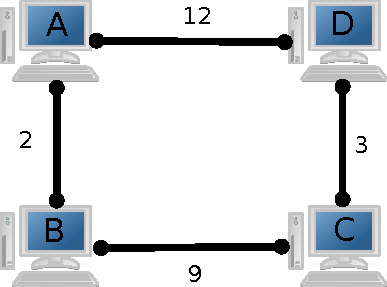
\includegraphics[scale=0.6]{img/algorithms/SAT_match}
  \label{figure:sat_match:before}
}\qquad\qquad
\subfigure[(left) A jumps to B in order to match the logical topology to the
physical. (right) State of the logical topology after the jump.] {
  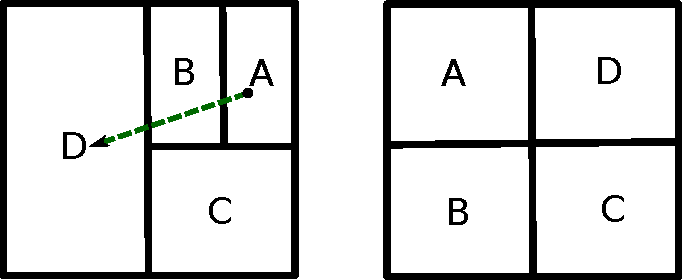
\includegraphics[scale=0.6]{img/algorithms/SAT_match2}
  \label{figure:sat_match:after}
}
\caption{The SAT-Match algorithm.}
\label{figure:sat_match}
\end{figure}

\emph{SAT-Match} \cite{ren_satmatch_2004}. Even though no theoretical proof is
given, valid results are obtained and demonstrated through experimentations.
Similar to the other approaches in the proximity neighbour selection,
\textit{SAT-Match} uses probing to detect close by peers and obtain proximity
information. However, as an additional feature, SAT-Match peers can do
selective jumps to adjust their positioning in the DHT, if it reduces the
\emph{stretch} of its one-hop neighbourhood. The paper defines stretch
$S = \frac{\bar{L_l}}{\bar{L_p}}$, where $\bar{L_l}$ is the average
logical link latency while the $\bar{L_p}$ is the average physical
link latency, and uses it a way quantify the \emph{topology
match degree} of the constructed overlay. For the probing phase SAT-Match uses a
small TTL value for the probing messages in order to reduce
redundancy\cite{jiang_lightflood_2008}. This process begins as soon as the node
joins the network using a DHT mechanism. Each probing message contains
information about the source and a small TTL value. The recipient of such a
message returns information about itself to the source and forwards the probing
message to its neighbours if the TTL is non-zero. The discovered nodes are
referred to as $TTL-k$ neighbourhood of the source node based on the $TTL$
distance to the source node. Blindly selecting the peer with the smallest RTT
as neighbour is, generally, not the optimal decision to make in order to achieve
global stretch reduction. In a structured scheme, when a node jumps to connect
to a physically close node, it may need to connect to other distant nodes to
maintain the structure's integrity, thus creating an overall increase in the
overlay's stretch. The two nodes with the smallest RTT are then used in order to
select one zone to jump in this phase. The algorithm is as follows: The source
node $S$ calculates the stretch change of its $TTL-1$ neighbourhood and that of
the $TTL-1$ neighbourhood of the first of the previously selected peers. These
calculations are made as if the jump has been made. If the stretch reduction is
over a predefined threshold the jump is performed, otherwise the second selected
candidate is picked and the same computations are performed. If again, the
threshold is not met, then no jump is ultimately done. In case of a jump, this
is performed as a combination of \emph{leave} and \emph{join} operations, in the
CAN context. Figure~\ref{figure:sat_match} demonstrates the selective jump on an
example topology.

%
%\paragraph{}
%Moreover the algorithm takes several issues into consiteration in order to
%  furtherly improve the resulted overlay. For example when multiple nodes try
% to jump simultaneously into a region, then the logical link brakes from one
% attempt may result in inacurate computation of the gain factor, for an other.
% This situation is identified as \emph{contention} and the nodes use an
% exponatial back-off algorithm to avoid it. An other problem is the uneseccary
% traffic incuerred by the probing phase in a region that after several jumps
% has settled to a stable state. In these cases it is more likely for jump
% attempts to be proven worthless. The algorithm doubles the probing period of
% such nodes, every time a jump is not taken.
%
%\paragraph{}
%The authors claim that this continuously adaptive mechanism achieves global
%  topology matching optimization in a sufficiently large scope. This also
% secures the fast adaptation to frequent network changes. It also considered
% lightweight and can easily be embedded into current p2p systems, as well
% as effectively combined with other techniques, such as landmark binning.

%
% TODO: SOME DISCUSSION
%
% It is reported that,
% due to the selective jumps, SAT-Match achieves $40\%$ reduction in
% link stretch, and when used with the landmark binning (see
% Sec. \ref{sec:landmark_binning}), the reduction rate increases up to $60\%$.
% For dynamic environments, with frequent node arrival and leave, SAT-Match
% scales much better than Mithos, due to its self adaptation mechanism and
% selective jumps.

\begin{center}
\begin{tabular}{ccc}
\emph{Efficiency} & \emph{Overhead} & \emph{Scalability} \\
\hline
% SAT-Match seems to outperform landmark binning in the sense of providing a
% higher grained differenciation of proximity, adding to the fact that
% SAT-match is fully distributed. Also to further enhance the efficiency it can
% work cooperatively with landmark binning itself.
high &
% distance probing and iterative computations add to the approach's overhead.
% Also the fact that the selective jumps are not always performed the added
% overhead to efficiency gained is not guarranteed in any configuration and
% circumstance.
medium &
% The self-adaptation nature of the algorithm and the selective jump mechanisms
% scale much better than, for example, Mithos.
medium
\end{tabular}
\end{center}

%%%%%%%%%%%%%%%%%%%%%%%%%%%%%%%%%%%%%%%%%%%%%%%%%%%%%%%%%%%%%%%%%%%%%%%%%%%%%%%%
\paragraph*{ \bf Delay Aware P2P System}
A new \emph{Delay Aware P2P System (DAPS)} is introduced in
\cite{zhang_daps_2005}. Its main goal is to reduce the time $L$ of a look-up
request by dividing the routing tables of peers into several sectors in
increasing delay. The source node emitting the query message defines a delay
boundary or the pruning factor $L_t$ in the paper's context. Request messages
will be forwarded only to nodes whose delay less than or equal to $L_t$. With
the clustered routing tables and the loose organisation the overlay network of
\emph{DAPS} is between structured and unstructured.

% TODO: MAYBE REVIEW THE EVALUATION
\begin{center}
\begin{tabular}{ccc}
\emph{Efficiency} & \emph{Overhead} & \emph{Scalability} \\
\hline
%
low &
%
low &
%
medium
\end{tabular}
\end{center}

%%%%%%%%%%%%%%%%%%%%%%%%%%%%%%%%%%%%%%%%%%%%%%%%%%%%%%%%%%%%%%%%%%%%%%%%%%%%%%%%
%%%%%%%%%%%%%%%%%%%%%%%%%%%%%%%%%%%%%%%%%%%%%%%%%%%%%%%%%%%%%%%%%%%%%%%%%%%%%%%%
\subsection{Discussion on the Algorithms for Structured Architectures}
%%%%%%%%%%%%%%%%%%%%%%%%%%%%%%%%%%%%%%%%%%%%%%%%%%%%%%%%%%%%%%%%%%%%%%%%%%%%%%%%
%%%%%%%%%%%%%%%%%%%%%%%%%%%%%%%%%%%%%%%%%%%%%%%%%%%%%%%%%%%%%%%%%%%%%%%%%%%%%%%%
Structured P2P network algorithms use a global distributed hash table or a
prefix tree structure to uniquely lookup peers or their data in the overlay
network. As all the data is kept within the overlay, each node behaves as a
client and a server, therefore nodes join and leave according to rules
determined by the integrity of the global data structure. The main advantage of
the structured P2P topology is that by the help of the global data structure,
peers or their data can be found within the network even if there is only a
single copy of that item present. However, each node join and leave creates
maintenance overhead for the network due to updates required by the global data
structure, and for networks with frequent node arrivals and departures the
topology uses valuable network resources just to update the global structure.
Nodes join the network by using a key value, which determines the location and
the neighbourhood of the new node within the network. However, assigning
random key values to the newly inserted nodes creates non-optimal matching with
the underlying physical network topology, therefore, increasing the overhead of
the network even more. One solution for handling the topology mismatch problem
is to consider the proximity of the peers when generating the key and joining
the node to the network, so that nodes within the same network domains are
selected as peers, or neighbours, during the overlay topology construction.

This section gathered together some of the most distinctive research work that
can be found in the literature for addressing the inefficient network resource
utilisation in structured architectures imposed by the topology mismatch
problem. A categorisation of the methods used for achieving their goals is the
following based on previous work from
\cite{castro_proximitydht_2002,castro_topawareroute_2002,ratnasamy_openq_2002}:
\begin{inparaenum}[\itshape i\upshape)]
  \item geographic-layout-based,
  \item proximity-routing-based,
  \item proximity neighbour selection based,
\end{inparaenum}

A quick overview can be obtained in Table~\ref{structured:table}. Topology
adaptation, landmarking and caching/replication have been visited during the
discussion on unstructured systems in Section~\ref{section:unstructured} so
we will not elaborate more here. Again, we additionaly gather highlights and a
rough estimation of each algorithm's positive and negative aspects regarding
their implementation.

% \renewcommand\arraystretch{1.1}

\begin{landscape}
%\begin{figure}[h!]
\hspace{-3ex}
\begin{center}
\footnotesize
%\begin{tabular}{
\begin{longtable}{
m{2cm}
m{1cm}
m{1cm}
m{1cm}
m{1cm}
m{1cm}
m{1cm}
m{3cm}
m{5cm}
}
%|>{\columncolor[gray]{.7}}m{0.15\columnwidth}
%|>{\columncolor[gray]{.9}}m{0.05in}
%|>{\columncolor[gray]{.8}}m{0.05\columnwidth}
%|>{\columncolor[gray]{.9}}m{0.05\columnwidth}
%|>{\columncolor[gray]{.9}}m{0.05\columnwidth}
%|>{\columncolor[gray]{.8}}m{0.05\columnwidth}
%|>{\columncolor[gray]{.9}}m{0.05\columnwidth}
%|>{\columncolor[gray]{.8}}m{0.1\columnwidth}
%|>{\columncolor[gray]{.9}}m{0.1\columnwidth}
%|>{\columncolor[gray]{.8}}m{0.1\columnwidth+}
%|
%}
\caption[Summary table for structured algorithms]{Summary table for structured algorithms.} \label{structured:table} \\
\hline
%%%%%%%%%%%%%%%%%%%%%%%%%%%%%%%%%%%%%%%%%%%%%%%%%%%%%%%%%%%%%%%%%%%%%%%%%%%%%%%%
% first head
\rowcolor[gray]{.5}
\textbf{Algorithm / Paper} &
\textbf{Topology Adaptation} &
\textbf{Landmarking} &
\textbf{Proximity Routing} &
\textbf{Proximity Neighbour Selection} &
\textbf{Geographic Layout} &
\textbf{Caching / Replication} &
\textbf{Highlights} &
\textbf{Pros / Cons}\\
\hline
\endfirsthead
%%%%%%%%%%%%%%%%%%%%%%%%%%%%%%%%%%%%%%%%%%%%%%%%%%%%%%%%%%%%%%%%%%%%%%%%%%%%%%%%
% subsequent heads
\multicolumn{9}{c}%
{\tablename\ \thetable\ -- \textit{Continued from previous page}} \\
\hline
\rowcolor[gray]{.5}
\textbf{Algorithm / Paper} &
\textbf{Topology Adaptation} &
\textbf{Landmarking} &
\textbf{Proximity Routing} &
\textbf{Proximity Neighbour Selection} &
\textbf{Geographic Layout} &
\textbf{Caching / Replication} &
\textbf{Highlights} &
\textbf{Pros / Cons}\\
\hline
\endhead
%%%%%%%%%%%%%%%%%%%%%%%%%%%%%%%%%%%%%%%%%%%%%%%%%%%%%%%%%%%%%%%%%%%%%%%%%%%%%%%%
% foot
\hline \multicolumn{9}{r}{\textit{Continued on next page}} \\
\endfoot
%%%%%%%%%%%%%%%%%%%%%%%%%%%%%%%%%%%%%%%%%%%%%%%%%%%%%%%%%%%%%%%%%%%%%%%%%%%%%%%%
% last foot
\hline
\endlastfoot
%%%%%%%%%%%%%%%%%%%%%%%%%%%%%%%%%%%%%%%%%%%%%%%%%%%%%%%%%%%%%%%%%%%%%%%%%%%%%%%%
% data
\textbf{Global Soft-State} &
{\large \CheckedBox} &
{\large \CheckedBox} &
{\large \Square} &
{\large \Square} &
{\large \CheckedBox} &
{\large \Square} &
\begin{tabular}[l]{m{3cm}}
Hybrid landmark binning.\\
Probing scheme for proximity detection.\\
Strategic injection of proximity info around the network.\\
Subscription-notification system to dynamically adapt to network changes.
\end{tabular} &
\begin{tabular}[l]{m{5cm}}
+ Greatly reduces routing latency to far away nodes.\\
-- Host state maintenance.\\
-- Unable to identify nodes that are close to routers/gateways.\\
-- Its static nature sacrifices the self-organising attribute of DHTs.
\end{tabular}
\\
\hline
%%%%%%%%%%%%%%%%%%%%%%%%%%%%%%%%%%%%%%%%%%%%%%%%%%%%%%%%%%%%%%%%%%%%%%%%%%%%%%%%
\textbf{Mithos} &
{\large \Square} &
{\large \Square} &
{\large \CheckedBox} &
{\large \Square} &
{\large \CheckedBox} &
{\large \Square} &
\begin{tabular}[l]{m{3cm}}
Directed incremental probing.\\
Synthetic coordinates.
\end{tabular} &
\begin{tabular}[l]{m{5cm}}
-- Does not effectively manage dynamic peer arrival and leave.
\end{tabular}
\\
\hline
%%%%%%%%%%%%%%%%%%%%%%%%%%%%%%%%%%%%%%%%%%%%%%%%%%%%%%%%%%%%%%%%%%%%%%%%%%%%%%%%
\textbf{LAPTOP} &
{\large \CheckedBox} &
{\large \Square} &
{\large \Square} &
{\large \Square} &
{\large \CheckedBox} &
{\large \CheckedBox} &
\begin{tabular}[l]{m{3cm}}
Tree-based hierarchy.
\end{tabular} &
\begin{tabular}[l]{m{5cm}}
+ Reduces hops during message routing.\\
+ Minimal maintenance overhead.\\
-- Heartbeat approach incurs overhead even when not needed.
\end{tabular}
\\
\hline
%%%%%%%%%%%%%%%%%%%%%%%%%%%%%%%%%%%%%%%%%%%%%%%%%%%%%%%%%%%%%%%%%%%%%%%%%%%%%%%%
\textbf{Landmark Binning} &
{\large \Square} &
{\large \CheckedBox} &
{\large \Square} &
{\large \Square} &
{\large \CheckedBox} &
{\large \Square} &
Binning &
\\
\hline
%%%%%%%%%%%%%%%%%%%%%%%%%%%%%%%%%%%%%%%%%%%%%%%%%%%%%%%%%%%%%%%%%%%%%%%%%%%%%%%%
\textbf{Proximity in Kademlia} &
{\large \CheckedBox} &
{\large \Square} &
{\large \CheckedBox} &
{\large \CheckedBox} &
{\large \Square} &
{\large \Square} &
\begin{tabular}[l]{m{3cm}}
% Replacing XOR metric with a function that minimises the underlying cost.\\
% Clustering (MaxMind geolocation technology).
\end{tabular} &
\begin{tabular}[l]{m{5cm}}
+ Proximity routing works in Kademlia to improve connection locality.
\end{tabular}
\\
\hline
%%%%%%%%%%%%%%%%%%%%%%%%%%%%%%%%%%%%%%%%%%%%%%%%%%%%%%%%%%%%%%%%%%%%%%%%%%%%%%%%
\textbf{CHOP6} &
{\large \Square} &
{\large \Square} &
{\large \CheckedBox} &
{\large \Square} &
{\large \Square} &
{\large \Square} &
\begin{tabular}[l]{m{3cm}}
Ipv6 format exploitation.\\
Additional RTT information.
\end{tabular} &
\\
\hline
%%%%%%%%%%%%%%%%%%%%%%%%%%%%%%%%%%%%%%%%%%%%%%%%%%%%%%%%%%%%%%%%%%%%%%%%%%%%%%%%
\textbf{T2MC} &
{\large \Square} &
{\large \CheckedBox} &
{\large \CheckedBox} &
{\large \Square} &
{\large \Square} &
{\large \Square} &
\begin{tabular}[l]{m{3cm}}
Clusterting using traceroute logs.
\end{tabular} &
\begin{tabular}[l]{m{5cm}}
+ Prioritise interaction of peers and edge gateways.\\
-- Extended overhead.\\
-- Traceroute is sometimes disabled by ISPs.
\end{tabular}
\\
\hline
%%%%%%%%%%%%%%%%%%%%%%%%%%%%%%%%%%%%%%%%%%%%%%%%%%%%%%%%%%%%%%%%%%%%%%%%%%%%%%%%
\textbf{PChord} &
{\large \Square} &
{\large \Square} &
{\large \CheckedBox} &
{\large \Square} &
{\large \Square} &
{\large \Square} &
\begin{tabular}[l]{m{3cm}}
Maintenance of a proximity list.
\end{tabular} &
\begin{tabular}[l]{m{5cm}}
+ Dynamic maintenance of the proximity list.\\
+ Reduces routing costs.\\
+ Can constrain constly jumps in and out of network partitions.\\
+ Maintenance cost kept to a minimal (node join/leave heartbeat for lists)
\end{tabular}
\\
\hline
%%%%%%%%%%%%%%%%%%%%%%%%%%%%%%%%%%%%%%%%%%%%%%%%%%%%%%%%%%%%%%%%%%%%%%%%%%%%%%%%
\textbf{AChord} &
{\large \Square} &
{\large \Square} &
{\large \CheckedBox} &
{\large \Square} &
{\large \Square} &
{\large \Square} &
\begin{tabular}[l]{m{3cm}}
Exploits IPv6's anycast mechanism.
\end{tabular} &
\begin{tabular}[l]{m{5cm}}
+ Releaved from the bootstrapping process.\\
+ Easy to implement (just the additional neighbourhood table).
\end{tabular}
\\
\hline
%%%%%%%%%%%%%%%%%%%%%%%%%%%%%%%%%%%%%%%%%%%%%%%%%%%%%%%%%%%%%%%%%%%%%%%%%%%%%%%%
\textbf{Chord6} &
{\large \Square} &
{\large \Square} &
{\large \CheckedBox} &
{\large \Square} &
{\large \Square} &
{\large \Square} &
\begin{tabular}[l]{m{3cm}}
Exploits IPv6's hierarchical features.
\end{tabular} &
\begin{tabular}[l]{m{5cm}}
+ Reduces inter-domain traffic between ISPs.\\
+ Easily portable to other DHTs.\\
-- It cannot distinguish between close by domains in order to identify the best
next hop when an interdomain step must be taken.
\end{tabular}
\\
\hline
%%%%%%%%%%%%%%%%%%%%%%%%%%%%%%%%%%%%%%%%%%%%%%%%%%%%%%%%%%%%%%%%%%%%%%%%%%%%%%%%
\textbf{DHT-PNS} &
{\large \Square} &
{\large \Square} &
{\large \Square} &
{\large \CheckedBox} &
{\large \Square} &
{\large \Square} &
\begin{tabular}[l]{m{3cm}}
Grouping through synthetic coordinates.\\
Partitioning using a concentric cycle clustering scheme.
\end{tabular} &
\begin{tabular}[l]{m{5cm}}
-- It assumes uniform node distribution which is not always the case in a synthetic coordinate system.\\
-- Clustering nodes might be a single point of failure.
\end{tabular}
\\
\hline
%%%%%%%%%%%%%%%%%%%%%%%%%%%%%%%%%%%%%%%%%%%%%%%%%%%%%%%%%%%%%%%%%%%%%%%%%%%%%%%%
\textbf{Quasi-Chord} &
{\large \Square} &
{\large \CheckedBox} &
{\large \Square} &
{\large \CheckedBox} &
{\large \Square} &
{\large \Square} &
\begin{tabular}[l]{m{3cm}}
Geometric space coordinates (GNP)\\
Transformation of the coordinate space into 1-d Cantor space for easier mapping to the Chord hierarchy\\
Two finger tables (clockwise, anti-clockwise)
\end{tabular} &
\begin{tabular}[l]{m{5cm}}
-- Not fully distributed (GNP is landmark based).\\
-- Makes an indirect assumption of a maximum number of allowable hosts.\\
-- Doubles the required routing information which needs to be created and maintained.
\end{tabular}
\\
\hline
%%%%%%%%%%%%%%%%%%%%%%%%%%%%%%%%%%%%%%%%%%%%%%%%%%%%%%%%%%%%%%%%%%%%%%%%%%%%%%%%
\textbf{IPBC} &
{\large \Square} &
{\large \Square} &
{\large \Square} &
{\large \CheckedBox} &
{\large \Square} &
{\large \Square} &
\begin{tabular}[l]{m{3cm}}
IP address prefixes (16 bit for IPv4) to detect proximity.
\end{tabular} &
\begin{tabular}[l]{m{5cm}}
+ Prefix is stored in the DHT so the proximity identification becomes as easy as to query the prefix.\\
+ DHT maintenance mechanisms for both volunteer or falure departures of peers.\\
-- Performance/accuracy tradeoff in choosing the prefix length to be used.
\end{tabular}
\\
\hline
%%%%%%%%%%%%%%%%%%%%%%%%%%%%%%%%%%%%%%%%%%%%%%%%%%%%%%%%%%%%%%%%%%%%%%%%%%%%%%%%
\textbf{Cone} &
{\large \Square} &
{\large \CheckedBox} &
{\large \Square} &
{\large \CheckedBox} &
{\large \Square} &
{\large \Square} &
\begin{tabular}[l]{m{3cm}}
2-layer ID space.\\
Group concept for dividing nodes according to a common Chord id prefix.
\end{tabular} &
\begin{tabular}[l]{m{5cm}}
+ The first step of the routing scheme exploits proximity thus reducing message exchange costs.\\
-- Not fully distributed as it relies on landmarks.\\
-- Maintenance of three routing tables is needed.
\end{tabular}
\\
\hline
%%%%%%%%%%%%%%%%%%%%%%%%%%%%%%%%%%%%%%%%%%%%%%%%%%%%%%%%%%%%%%%%%%%%%%%%%%%%%%%%
\textbf{DynaMo} &
{\large \Square} &
{\large \CheckedBox} &
{\large \Square} &
{\large \CheckedBox} &
{\large \Square} &
{\large \Square} &
\begin{tabular}[l]{m{3cm}}
Random Landmarking (RLM).\\
Closest Neighbour Prefix Assignment (CPNA).\\
Making last hop as local as possible.
\end{tabular} &
\begin{tabular}[l]{m{5cm}}
+ Developed with mobile, ad-hoc networks in mind.\\
+ Evenly distributed IDs.\\
+ Dynamic landmarking is a fully distributed approach.\\
-- RLM imposes extra network stress especially to landmark nodes.\\
-- CPNA is a coarse-grained proximity approach.
\end{tabular}
\\
\hline
%%%%%%%%%%%%%%%%%%%%%%%%%%%%%%%%%%%%%%%%%%%%%%%%%%%%%%%%%%%%%%%%%%%%%%%%%%%%%%%%
\textbf{SAT-Match} &
{\large \Square} &
{\large \Square} &
{\large \Square} &
{\large \CheckedBox} &
{\large \Square} &
{\large \Square} &
\begin{tabular}[l]{m{3cm}}
Selective jumps to adjust peer positioning in the DHT.\\
Stretch reduction scheme.
\end{tabular} &
\begin{tabular}[l]{m{5cm}}
+ Continuously adaptive mechanism.\\
+ It can be considered lightweight.\\
+ Can coexist with other approaches (like landmarking).\\
+ Works sufficiently for large scopes as well as environments with high churn.\\
+ Compared to Mithos scales much better.\\
-- Contention situation in selective jump phase.\\
-- Probing phase incurs unnecessary traffic.
\end{tabular}
\\
\hline
%%%%%%%%%%%%%%%%%%%%%%%%%%%%%%%%%%%%%%%%%%%%%%%%%%%%%%%%%%%%%%%%%%%%%%%%%%%%%%%%
\textbf{Delay Aware P2P System} &
? &
? &
? &
? &
? &
? &
? &
?
\\
\hline
%%%%%%%%%%%%%%%%%%%%%%%%%%%%%%%%%%%%%%%%%%%%%%%%%%%%%%%%%%%%%%%%%%%%%%%%%%%%%%%%

% \hline
% \textbf{Global Softstate} &
% \textbf{Geographic layout} Uses first landmark clustering
% then measures RTTs to identify close nodes &  &  \\

% \hline
% \textbf{Mithos} &
% \textbf{Geographic layout} Uses nodes as topology landmarks and directed
% incremental probing to optimize topology & & Scales well as all
% operations are local ??? \\
% 
% \hline
% \textbf{Self-Adaptive Topology Matching} &
% \textbf{Proximity neighbour selection} Uses lightweight probing and
% selective jumps to optimize the topology & CAN &  Better than Mithos \\

% \hline
% \textbf{Delay Aware P2P System} & \textbf{} & & \\

% \hline
% \textbf{VERSION OF CHORD - DHT-PNS} &
% \textbf{Proximity neighbour selection} Uses Proximity Neighbour Selection and the Vivaldi
% system & Chord  &  \\

% \hline
% \textbf{MAY OMIT- VERSION OF CHORD - Quasi-Chord} &
% \textbf{Proximity based}  & Chord  &  \\

% \hline
% \textbf{LAPTOP} &
% \textbf{Geographic layout} Hierarchical overlay structure  &  & routing path length $\log{_d N}$,
% join/leave overhead $d\log{_d N}$ \\

% \hline
% \textbf{IP-Based Clustering} &
% \textbf{Proximity neighbour selection} Proximity neighbour selection based on longest common
% prefix of IP addresses &    &  \\

% \hline
% \textbf{CHOord considering Proximity on IPv6} &
% \textbf{Proximity routing} Uses IPv6 address format to provide proximity &  Chord
%  & Better than Chord \\

% \hline
% \textbf{Proximity in Kademlia} &
% \textbf{Proximity routing} Applies  proximity neighbour selection (PNS) and proximity route selection (PRS)
% to Kademlia & Kademlia &   \\

% \hline
% \textbf{Cone} &
% \textbf{Proximity neighbour selection} Uses proximity neighbour selection (PNS) & Chord  & Better than Chord \\

% \hline
% \textbf{DynaMO} &  &  &  \\
% 
% \hline
% \textbf{MAY OMIT-BADLY WRITTEN-PChord} &
% \textbf{Proximity based}  &  Chord  & \\
% 
% \hline
% \textbf{AChord} &  & & \\

% \hline
% \textbf{Chord6} &
% \textbf{Proximity routing} Uses IPv6 hierarchical address format to cluster
% topologically close nodes & Chord  &  \\

% \hline
\end{longtable}
\end{center}
\vspace{-2.5ex}
\vspace{-2.5ex}
%\label{fig:struct_compare_table}
%\end{figure}
 \end{landscape}


%%%%%%%%%%%%%%%%%%%%%%%%%%%%%%%%%%%%%%%%%%%%%%%%%%%%%%%%%%%%%%%%%%%%%%%%%%%%%%%%
%%%%%%%%%%%%%%%%%%%%%%%%%%%%%%%%%%%%%%%%%%%%%%%%%%%%%%%%%%%%%%%%%%%%%%%%%%%%%%%%
%                               STRUCTURED
%%%%%%%%%%%%%%%%%%%%%%%%%%%%%%%%%%%%%%%%%%%%%%%%%%%%%%%%%%%%%%%%%%%%%%%%%%%%%%%%
%%%%%%%%%%%%%%%%%%%%%%%%%%%%%%%%%%%%%%%%%%%%%%%%%%%%%%%%%%%%%%%%%%%%%%%%%%%%%%%%

%\pgfplotsset{width=7cm,compat=newest}
\onecolumn

%%%%%%%%%%%%%%%%%%% EFFICIENCY %%%%%%%%%%%%%%%%%%%
\begin{figure}[ht]
\centering
\resizebox{\textwidth}{!}{%
%\begin{landscape}
%\begin{center}
\begin{tikzpicture}
\begin{axis}[
  xbar,
  bar width=7pt,
  xlabel=\emph{Efficiency},
  ylabel=\emph{Algorithm},
  symbolic x coords={low, medium, high},
  symbolic y coords={
    SATMatch,
    3DO,
    DynaMOCNPA,
    DynaMORLM,
    %Cone,
    IPBC,
    QuasiChord,
    DHTPNS,
    Chord6,
    AChord,
    PChord,
    T2MC,
    CHOP6,
    ProximityInKademlia,
    %Landmark Binning,
    LAPTOP,
    Mithos,
    GlobalSoftState
  },
  every axis y label/.style=
    {at={(ticklabel cs:0.5)},rotate=90,anchor=near ticklabel},
%   x tick label style={rotate=45,anchor=east},
  xtick=data, ytick=data,
%   ymin=low,ymax=high,ytickmin=low,
  height=\textheight - 0.3cm,
  width=\textwidth,
  enlargelimits=0.05,
%  title=\emph{Efficiency} Pictorial Comparison of Structured Approaches.
]

\addplot[black,fill=gray!20, postaction={pattern=north east lines}]
table[x=EFFICIENCY,y=ALGORITHM]
{structured-plot.dat};

\end{axis}
\end{tikzpicture}
}
\caption{\emph{Efficiency} Pictorial Comparison of Structured Approaches.}
\label{structured:plot:efficiency}
\end{figure}
%\end{center}
%\end{landscape}

%%%%%%%%%%%%%%%%%%% OVERHEAD %%%%%%%%%%%%%%%%%%%
\begin{figure}[ht]
\centering
\resizebox{\textwidth}{!}{%
%\begin{landscape}
%\begin{center}
\begin{tikzpicture}
\begin{axis}[
  xbar,
  bar width=7pt,
  xlabel=\emph{Overhead},
  ylabel=\emph{Algorithm},
  symbolic x coords={low, medium, high},
  symbolic y coords={
    SATMatch,
    3DO,
    DynaMOCNPA,
    DynaMORLM,
    %Cone,
    IPBC,
    QuasiChord,
    DHTPNS,
    Chord6,
    AChord,
    PChord,
    T2MC,
    CHOP6,
    ProximityInKademlia,
    %Landmark Binning,
    LAPTOP,
    Mithos,
    GlobalSoftState
  },
  every axis y label/.style=
    {at={(ticklabel cs:0.5)},rotate=90,anchor=near ticklabel},
%   x tick label style={rotate=45,anchor=east},
  xtick=data, ytick=data,
%   ymin=low,ymax=high,ytickmin=low,
  height=\textheight - 0.3cm,
  width=\textwidth,
  enlargelimits=0.05,
%  title=\emph{Overhead} Pictorial Comparison of Structured Approaches.
]

\addplot[black,fill=gray!20, postaction={pattern=crosshatch}]
table[x=OVERHEAD,y=ALGORITHM]
{structured-plot.dat};

\end{axis}
\end{tikzpicture}
}
\caption{\emph{Overhead} Pictorial Comparison of Structured Approaches.}
\label{structured:plot:overhead}
\end{figure}
%\end{center}
%\end{landscape}

%%%%%%%%%%%%%%%%%%% SCALABILITY %%%%%%%%%%%%%%%%%%%
\begin{figure}[ht]
\centering
\resizebox{\textwidth}{!}{%
%\begin{landscape}
%\begin{center}
\begin{tikzpicture}
\begin{axis}[
  xbar,
  bar width=7pt,
  xlabel=\emph{Scalability},
  ylabel=\emph{Algorithm},
  symbolic x coords={low, medium, high},
  symbolic y coords={
    SATMatch,
    3DO,
    DynaMOCNPA,
    DynaMORLM,
    %Cone,
    IPBC,
    QuasiChord,
    DHTPNS,
    Chord6,
    AChord,
    PChord,
    T2MC,
    CHOP6,
    ProximityInKademlia,
    %Landmark Binning,
    LAPTOP,
    Mithos,
    GlobalSoftState
  },
  every axis y label/.style=
    {at={(ticklabel cs:0.5)},rotate=90,anchor=near ticklabel},
%   x tick label style={rotate=45,anchor=east},
  xtick=data, ytick=data,
%   ymin=low,ymax=high,ytickmin=low,
  height=\textheight - 0.3cm,
  width=\textwidth,
  enlargelimits=0.05,
%  title=\emph{Scalability} Pictorial Comparison of Structured Approaches.
]

\addplot[black,fill=gray!50, postaction={pattern=crosshatch dots}]
table[x=SCALABILITY,y=ALGORITHM]
{structured-plot.dat};

\end{axis}
\end{tikzpicture}
}
\caption{\emph{Scalability} Pictorial Comparison of Structured Approaches.}
\label{structured:plot:scalability}
\end{figure}
%\end{center}
%\end{landscape}

\twocolumn


%%%%%%%%%%%%%%%%%%%%%%%%%%%%%%%%%%%%%%%%%%%%%%%%%%%%%%%%%%%%%%%%%%%%%%%%%%%%%%%%
\subsubsection{Geographic layout} \label{section:geographic_layout}
Inside geographic layout category fall those kind of methods which practically
position physically close by nodes together in the application space as well.
This is done by adjusting and maintaining the routing tables of all involved
peers accordingly by exploiting proximity information that describe the overall
geographic positioning of the peer nodes. Landmark servers and RTT measurements
are two popular methods, which can also be used in conjunction, to discover
physically close by peers over the network. However, as discussed in Section
\ref{sec:landmark_binning}, these methods do not always give reliable estimates
for the node positions over the internet. The landmark servers are not
self-organizing and have maintenance overheads. To serve a P2P network with
millions of peers, multiple landmark servers distributed over the whole world is
required, which is hard to manage. The RTT measurements also can measure the
delay between peers, but it is a greedy method, which can result non-optimal
overlay topologies especially if close by nodes have low bandwidth connections
among themselves.

Even though managing the overlay structure based on the geographic layout of the
nodes improves the query efficiency of the system, on the other hand, it tends
to create hotspots, and the needed failure resilience is undermined by the fact
that close by nodes are more likely to suffer collective failures.


%%%%%%%%%%%%%%%%%%%%%%%%%%%%%%%%%%%%%%%%%%%%%%%%%%%%%%%%%%%%%%%%%%%%%%%%%%%%%%%%
%
% TODO: Geographic Layout
%
%\begin{itemize}
% \item Geographic Layout\\
%The node IDs are assigned in such a way that nodes close by in the physical
%network topology, be close in the node ID space as well. Implementations that
%work relatively well with this approach have been incorporated into CAN. Nodes
%measure the RTT between themselves and a set of landmarks in order to match the
%CAN space as much as possible to the physical one. Unfortunately, the approach
%requires well known landmark servers and for that matter is  not fully
%self-organizing which can further lead to imbalanced node distribution. On
%other DHTs, such as Chord or Pastry, another problem emerges.  To gain fault
%tolerant properties, these protocols, replicate key-value pairs on neighbouring
%(in the ID space) nodes. When a proximity-based node ID assignment has been
%used, the needed failure resilience is undermined by the fact that close by
%nodes are more likely to suffer collective failures.
%

%%%%%%%%%%%%%%%%%%%%%%%%%%%%%%%%%%%%%%%%%%%%%%%%%%%%%%%%%%%%%%%%%%%%%%%%%%%%%%%%
\subsubsection{Proximity Routing}
Proximity routing does not require routing tables to be built using any
knowledge about network proximity. On the other hand it exploits such knowledge
in order to choose the best next hop during routing a message. This approach
tries to balance between choosing the node that will further progress the
routing towards the destination and choosing the closest entry in the routing
table, in terms of network proximity. As this is very difficult to be achieved,
the system might end up using a greedy approach that selects low latency paths
over the overlay, which maps to suboptimal longer paths on the physical
topology. Thus, in general, proximity neighbour selection is considered as a
superior method to proximity routing, however, joint uses of these two protocols
are also possible. Moreover, they are considered relatively less effective than
geographical layout when applied to CAN(-like) implementations. Moreover, the
technique has been incorporated into a version of Chord causing an increase on
the overhead of node joins and the size as well as maintenance cost of finger
tables.

%
%\cite{dabek_cfs_2001} proposes a server selection scheme for the Chord DHT, on
%the domain of proximity routing selection. In \emph{CFS}, each node predicts
%the entire lookup latency as a function of the total number of nodes and the
%average overlay next routing peer. The problem is that it is very difficult to
%have a clear picture on the total number of nodes and the average hop latency
%from the local. This leads to rough estimations that consequently decreases
%overall performance.
%

%%%%%%%%%%%%%%%%%%%%%%%%%%%%%%%%%%%%%%%%%%%%%%%%%%%%%%%%%%%%%%%%%%%%%%%%%%%%%%%%
\subsubsection{Proximity neighbour selection}
\emph{Proximity Neighbour Selection} constructs the routing tables using
proximity knowledge. The proximity information used in this method is different
than the landmark based systems described in
Section~\ref{section:geographic_layout}, as time-to-live values between nodes,
or directly node ID prefixes are used to detect proximity. Tapestry, Pastry, and
CAN successfully implemented the proximity into their algorithms by using this
approach. The routing protocol in Pastry is based on longest node ID prefix
matching, while CAN uses RTT values to detect close by nodes.
\cite{castro_proximityp2p_2002} reports that proximity neighbour selection as an
effective proximity based method.
